\documentclass[10pt]{beamer}
\usefonttheme{professionalfonts,serif}
\def\newblock{\hskip .11em plus .33em minus .07em}
\usepackage[numbers,sort]{natbib}
\renewcommand{\rmdefault}{psbx}
\usepackage[utf8]{inputenc}
\usepackage[T1]{fontenc}
\usepackage{textcomp}
\usepackage{eulervm}

\usetheme{default}           % tips from David Blei
\useinnertheme{circles}
\useoutertheme{infolines}
\setbeamertemplate{headline}{}
\setbeamertemplate{navigation symbols}{}
\setbeamerfont{itemize/enumerate subbody}{size=\normalsize}
\setbeamerfont{itemize/enumerate subsubbody}{size=\normalsize}
\usecolortheme{seahorse}
\setbeamersize{text margin left=2mm,text margin right=2mm}

\graphicspath{{../../figures/}}

\definecolor{mypine}{rgb}{0.05,0.45,0.05}
\definecolor{mycyan}{rgb}{0.0,0.9,0.9}
\newcommand{\Red}{\textcolor{red}}
\newcommand{\Blue}{\textcolor{blue}}
\newcommand{\Green}{\textcolor{mypine}}
\newcommand{\PineGreen}{\textcolor{mypine}}
\newcommand{\Magenta}{\textcolor{magenta}}
\newcommand{\Cyan}{\textcolor{mycyan}}

\newcommand{\N}{\mathcal{N}}
\newcommand{\R}{\mathbb{R}}
\newcommand{\T}{{\scriptsize^{\top}}}
\newcommand{\D}{\mathcal{D}}
\newcommand{\F}{\mathcal{F}}
\newcommand{\E}{\mathbb{E}}
\newcommand{\V}{\mathbb{V}}
\newcommand{\M}{\mathcal{M}}
\newcommand{\KL}{\mathcal{KL}}
\newcommand{\cut}[1]{}
\newcommand{\trace}{\operatorname{trace}}

\newcommand{\bmu}{{\boldsymbol{\mu}}}
\newcommand{\btheta}{\boldsymbol{\theta}}
\newcommand{\bepsilon}{\boldsymbol{\epsilon}}
\newcommand{\balpha}{\boldsymbol{\alpha}}
\newcommand{\bbeta}{\boldsymbol{\beta}}
\newcommand{\bphi}{\boldsymbol{\phi}}
\newcommand{\bPhi}{\boldsymbol{\Phi}}
\newcommand{\bSigma}{\boldsymbol{\Sigma}}
\newcommand{\bpi}{\boldsymbol{\pi}}
\newcommand{\blambda}{\boldsymbol{\lambda}}

\newcommand{\argmax}{\operatorname{argmax}}
\newcommand{\argmin}{\operatorname{argmin}}
\newcommand{\ci}{{\bot\negthickspace\negthickspace\bot}} % conditional indep.
\newcommand{\neigh}{\operatorname{ne}}
\newcommand{\vectr}[2]{  \left[ \!\!\begin{array}{c} #1 \\
      #2 \end{array} \!\!\right]}
\newcommand{\deff}{\stackrel{\mathrm{def}}{=}}
\newcommand{\deldel}[2]{\frac{\partial #1}{\partial #2}}

\newcommand{\maketilde}{\raisebox{0.4ex}{\tiny $\sim$}}
\newcommand{\bfa}{\mathbf a}
\newcommand{\bfb}{\mathbf b}
\newcommand{\bfe}{\mathbf e}
\newcommand{\bff}{\mathbf f}
\newcommand{\bfk}{\mathbf k}
\newcommand{\bfm}{\mathbf m}
\newcommand{\bfn}{\mathbf n}
\newcommand{\bfp}{\mathbf{p}}
\newcommand{\bfs}{\mathbf s}
\newcommand{\bfu}{\mathbf u}
\newcommand{\bfx}{\mathbf x}
\newcommand{\bfy}{\mathbf y}
\newcommand{\bft}{\mathbf t}
\newcommand{\bfv}{\mathbf v}
\newcommand{\bfw}{\mathbf w}
\newcommand{\bfA}{\mathbf A}
\newcommand{\bfI}{\mathbf I}
\newcommand{\bfK}{\mathbf K}


\title[Gaussian Densities]{(Multivariate) Gaussian (Normal)\\ Probability Densities}
\author[Rasmussen, Hern\`andez-Lobato \& Turner]{Carl Edward
  Rasmussen,  Jos\'e Miguel Hern\'andez-Lobato \& Richard Turner}
\date{April 20th, 2018}

\begin{document}

\begin{frame}
\titlepage
\end{frame}

\begin{frame}
\frametitle{Gaussian Density}

The probability density of a $D$-dimensional Gaussian with mean vector
$\boldsymbol{\mu}$ and covariance matrix $\Sigma$ is given by
%
\[
p({\bf x}|\boldsymbol{\mu},\Sigma)\;=\;
{\cal N}({\bf x}|\boldsymbol{\mu},\Sigma)\;=\;\frac{1}{(2\pi)^{D/2}|\Sigma|^{1/2}}
\exp\big(\!-\tfrac{1}{2}({\bf x}-\boldsymbol{\mu})^\top \Sigma^{-1}
({\bf x}-\boldsymbol{\mu})\big),
\]
%
and we also write
%
\[
{\bf x}|\boldsymbol{\mu},\Sigma\;\sim\;{\cal N}({\bf x}|\boldsymbol{\mu},\Sigma).
\]
%
The covariance matrix $\Sigma$ must be symmetric and positive definite.\\[1ex]

In the special (scalar) case where $D=1$ we have
%
\[
p(x|\mu,\sigma^2)\;=\;\frac{1}{\sqrt{2\pi\sigma^2}}
\exp\big(\!-\tfrac{1}{2}(x-\mu)^2/\sigma^2\big),
\]
%
where $\sigma^2$ is the variance and $\sigma$ is the standard deviation.\\[1ex]

The \emph{standard} Gaussian has $\boldsymbol{\mu}=\boldsymbol{0}$ and
$\Sigma=I$ (the unit matrix).
\end{frame}

\begin{frame}
\frametitle{Parametrisation}

There are two commonly used parametrisations of Gaussians
\begin{itemize}
\item \emph{standard} parametrisation:
\begin{itemize}
\item \emph{mean} $\boldsymbol{\mu}$ and
\item \emph{covariance} $\Sigma$
\end{itemize}
\item \emph{natural} parametrisation:
\begin{itemize}
\item \emph{natural mean}
  $\boldsymbol{\nu}=\Sigma^{-1}\boldsymbol{\mu}$ and
\item \emph{precision} matrix $R=\Sigma^{-1}$.
\end{itemize}
\end{itemize}
Different operations are more convenient in either parametrisation.

\end{frame}

\begin{frame}
\frametitle{Gaussian Pictures}

\end{frame}

\begin{frame}
\frametitle{Gaussian Properties}

Gaussians are closed both under marginalisation and conditioning.

If ${\bf x}$ and ${\bf y}$ are jointly Gaussian
\[
\left[\!\begin{array}{c}{\bf x}\\{\bf y}\end{array}\!\right] 
\]

\end{frame}

\begin{frame}
\frametitle{Kullback-Leibler Divergence (Relative Entropy)}

The Kullback-Leibler (KL) divergence between continuous distributions is
%
\[
{\cal KL}(q(x)||p(x))\;=\;\int q(x)\log\frac{q(x)}{p(x)}dx.
\]
%
The KL divergence is an asymmetric measure of distance between distributions.

The KL divergence between two Gaussians is
\[
{\cal KL}({\cal N}_0||{\cal N}_1)\;=\;\tfrac{1}{2}\log|\Sigma_1\Sigma_0^{-1}|
+\tfrac{1}{2}\operatorname{tr}\big(\Sigma_1^{-1}
\big((\boldsymbol{\mu}_0-\boldsymbol{\mu}_1)
(\boldsymbol{\mu}_0-\boldsymbol{\mu}_1)^\top + \Sigma_0 - \Sigma_1\big)\big).
\]

\end{frame}

\begin{frame}
\frametitle{KL matching constrained Gaussians}

It is often convenient to approximate one distribution with another,
simpler one, by finding the \emph{closest match} within a constrained family.\\[1ex]

Minimizing KL divergence between a \Green{general Gaussian ${\cal N}_g$} and a
factorized Gaussian ${\cal N}_f$ will match the means
$\boldsymbol\mu_f=\boldsymbol\mu_g$ and for the covariances either:
\[
\frac{\partial {\KL}(\Red{{\cal N}_f}||{\cal N}_g)}{\partial\Sigma_f}=
-\tfrac{1}{2}\Sigma_f^{-1}+\tfrac{1}{2}\Sigma_g^{-1}=0\;\Rightarrow\;
\Red{(\Sigma_f)_{ii} = 1/(\Sigma_g^{-1})_{ii}},
\]
or
\[
\frac{\partial {\KL}(\Blue{{\cal N}_g}||{\cal N}_f)}{\partial\Sigma_f}=
\tfrac{1}{2}\Sigma_f^{-1}-\tfrac{1}{2}\Sigma_f^{-1}\Sigma_g\Sigma_f^{-1}=0\;
\Rightarrow\;\Blue{(\Sigma_f)_{ii} = (\Sigma_g)_{ii}}.
\]
%
\parbox{0.7\linewidth}{
Interpretation:
\begin{itemize}
\item \Red{averaging wrt the \emph{factorized} Gaussian}, the fitted variance
equals the \Red{\emph{conditional} variance} of $\Green{\Sigma_g}$,
\item \Blue{averaging wrt the \emph{general} Gaussian}, the fitted variance
equals the \Blue{\emph{marginal} variance} of $\Green{\Sigma_g}$,
\end{itemize}
with straight forward generalization to block diagonal Gaussians.
}
\parbox{0.29\linewidth}{
\hfill
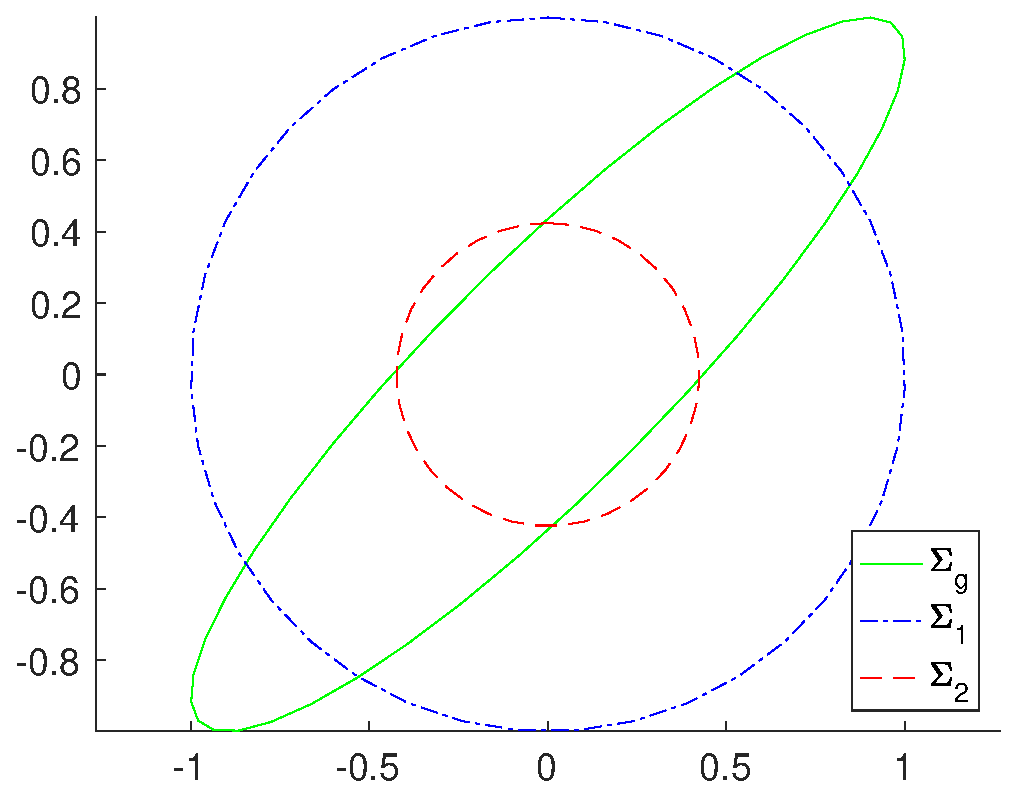
\includegraphics[width=\linewidth]{kl}
}

\end{frame}

\begin{frame}

\frametitle{Appendix: Some useful Gaussian identities}
If $x$ is multivariate Gaussian with mean $\mu$ and
covariance matrix $\Sigma$
\[
p({\bf x}; \mu, \Sigma)\;=\;(2\pi|\Sigma|)^{-D/2}\exp\big(-({\bf
    x}-\mu)^\top\Sigma^{-1}({\bf x}-\mu)/2\big),
\]
then
\[
\begin{split}
\E[{\bf x}]\;&=\;\mu,\\
\V[{\bf x}]\;&=\;\E[({\bf x}-\E[{\bf x}])^2]\;=\;\Sigma.
\end{split}
\]

For any matrix $A$, if ${\bf z} = A{\bf x}$ then ${\bf z}$ is Gaussian and
\[
\begin{split}
\E[{\bf z}] \;&=\; A\mu,\\
\V[{\bf z}] \;&=\;A\Sigma A^\top.
\end{split}
\]
\end{frame}

\begin{frame}
\frametitle{Matrix and Gaussian identities cheat sheet}

Matrix identities
\begin{itemize}
\item Matrix inversion lemma (Woodbury, Sherman \& Morrison formula)
%
\[
(Z+UWV^\top)^{-1}=Z^{-1}-Z^{-1}U(W^{-1}+V^\top Z^{-1}U)^{-1}V^\top Z^{-1}
\]
%
\item A similar equation exists for determinants
\[
|Z+UWV^\top|=|Z|\;|W|\;|W^{-1}+V^\top Z^{-1}U|
\]
\end{itemize}

The product of two Gaussian density functions
%
\[
\N(\bfx|{\mathbf a},A)\,\N(P^\top\,\bfx|{\mathbf b},B) = z_c\,
\N(\bfx|{\mathbf c},C)
\]
%
\vspace{-5mm}
\begin{itemize}
\item is proportional to a Gaussian density function with covariance and mean
%
\[
C = \left(A^{-1}+P\,B^{-1}P^\top\right)^{-1}\enspace \hspace{1cm} c =
C\,\left(A^{-1}{\mathbf a}+P\,B^{-1}\,{\mathbf b}\right)
\]
%
\item and has a normalizing constant $z_c$ that is Gaussian both in ${\mathbf
a}$ and in ${\mathbf b}$ 
%
\[
z_c = (2\,\pi)^{-\frac{m}{2}}|B+P^\top A\,P|^{-\frac{1}{2}}
\exp\big(-\frac{1}{2}({\mathbf b}-P^\top\,{\mathbf a})^\top
\left(B+P^\top A\,P\right)^{-1}({\mathbf b}-P^\top\,{\mathbf a})
\big)
\]
%
\end{itemize}
\end{frame}

\end{document}

